\documentclass[11pt,a4paper]{article}
\usepackage[margin=22mm]{geometry}
\usepackage[T1]{fontenc}
\usepackage{lmodern,graphicx,tabularx,booktabs,array,amsmath}
\usepackage[hidelinks]{hyperref}\urlstyle{same}
\setlength{\parindent}{0pt}
\setlength{\parskip}{5pt}
\setlength{\emergencystretch}{3em}
\newcolumntype{Y}{>{\raggedright\arraybackslash}X}
\graphicspath{{figures/}}
\newcommand{\diagram}[3]{\clearpage\section{#1}#2\begin{center}\includegraphics[width=\linewidth,height=.73\textheight,keepaspectratio]{#3}\end{center}}
\begin{document}
\begin{titlepage}
\centering
\vspace*{24mm}
{\Huge\bfseries CampusPool\par}
\vspace{7mm}
{\Large Campus Ride and Activity Coordination Website\par}
\vspace{14mm}
{\Large Final Project Report\par}
\vspace{5mm}
UCS503P Software Engineering\\
Academic year 2026--27
\vspace{19mm}

\begin{tabular}{@{}lr@{}}
\toprule
\textbf{Team member} & \textbf{Roll number}\\
\midrule
Pihu & 1024031014\\
Jayant Kaushik & 1024031016\\
Aashna & 1024031018\\
\bottomrule
\end{tabular}
\vfill
Department of Computer Science and Engineering\\
Thapar Institute of Engineering and Technology\\
Patiala
\end{titlepage}
{\small\tableofcontents}
\clearpage

\section{Abstract}
CampusPool is a campus-focused website for organising shared rides and finding company for non-travel activities. It provides searchable plans, join requests, organiser decisions and participation records. After a ride, the organiser records the actual fare and the website calculates equal shares. Riders can open a UPI link, acknowledge payment and wait for the organiser to confirm receipt.

The implementation uses a Next.js and TypeScript frontend, FastAPI backend and PostgreSQL database. Thapar email OTP sign-in controls account access, and WebSockets deliver live updates. This report explains the requirements, workflows, architecture, data model, design diagrams and verification approach. The original activity diagram is retained as a design-stage artifact, with the implemented account and payment behaviour explained alongside it.

\section{Introduction and problem statement}
Students travelling to railway stations, bus stands, airports or local destinations often seek others to share a cab or auto. Students also look for company for sports, walks, meals, movies and study sessions. Group chats support initial discussion, but messages can be buried and details can change without a clear record.

The coordination problem has several parts. A requester needs to find a plan at the right location and time. An organiser needs to decide who joins and track remaining capacity. Participants need to see whether a request is pending, accepted or rejected. After a ride, the group also needs a consistent calculation of each person's share.

CampusPool gives these interactions a defined workflow. A published plan contains its details, requests record interest and organiser decisions control membership. The completed ride produces a fare record that participants and the organiser can track.

\section{Objectives and scope}
The project aims to make plans discoverable, record participation decisions, preserve capacity limits and reduce manual fare calculation. It also provides communication and reporting controls for the campus community.

The implemented scope includes Thapar email account access, profiles, rides, activities, request management, fare tracking, UPI links, chat, notifications and administrative moderation. Users arrange their own vehicles. Payments occur in an external UPI application, and CampusPool records acknowledgement and confirmation. Activity participation has no associated fare-settlement step.

\clearpage
\section{Requirements}
\subsection{Functional requirements}
\begin{tabularx}{\linewidth}{@{}p{25mm}Y@{}}
\toprule
\textbf{Module} & \textbf{Required behaviour}\\
\midrule
Accounts & Accept an eligible Thapar email, send and validate an OTP, create a session and support profile management.\\[4pt]
Ride discovery & Publish rides with source, destination, departure, seat count and expected fare. Search and view available rides.\\[4pt]
Participation & Record a join request, let the organiser accept or reject it, and display the resulting status.\\[4pt]
Settlement & Complete a ride, record its actual fare, calculate shares and track rider acknowledgement and organiser confirmation.\\[4pt]
Activities & Publish and discover non-travel plans and manage join requests and participation.\\[4pt]
Communi-\newline cation & Provide chat for connected users and notifications about relevant updates.\\[4pt]
Moderation & Accept reports and support authorised administrative actions on users and posts.\\
\bottomrule
\end{tabularx}

\subsection{Quality requirements}
The interface should support phone and desktop use. Validation must run on the backend as well as in forms. Protected actions require an authenticated account and the appropriate organiser or administrator permission. Data should remain consistent when a request is retried or competing approvals target limited capacity.

Email and phone information should be controlled through the application's privacy settings. Secrets belong in environment configuration. Database migrations and container definitions support repeatable deployment. Performance and availability depend on the deployed infrastructure and require measurement under representative use.

\section{Account and participation workflow}
A user enters a Thapar email address and a one-time code delivered to that mailbox. The backend checks the code and establishes a session. Mailbox confirmation establishes access to the address. The current implementation does not query a university enrolment database.

For rides, the organiser enters pickup, destination, departure time, available seats and expected fare. A requester discovers the post and sends a request. The organiser accepts or declines it, and the requester sees the updated state. Accepted riders consume capacity. The backend must check permissions and capacity when applying a decision.

An activity follows a similar discover--request--decide workflow, using its title, category, location, start time and participant limit. Activities support coordination and completion without creating fare records.

\clearpage
\section{Fare splitting and payment tracking}
When the ride finishes, the organiser enters its actual fare. The fare is divided across the organiser and accepted riders.
\[
\text{Share per participant}=\frac{\text{Actual fare}}{\text{Total participants including organiser}}
\]
For INR~600 and four participants, the share is INR~150 each. The organiser has already paid the ride expense, so payment links are useful for the other riders who owe their shares.

A rider opens the UPI link and pays through an external application. The rider then marks the share as paid in CampusPool. This sets the acknowledgement flag. The organiser reviews receipt and confirms it, after which the payment record becomes \texttt{SUCCESS}. Until confirmation, the stored status remains \texttt{PENDING}. The website receives no automatic bank callback for this workflow.

\section{Architecture and implementation}
\subsection{Frontend}
Next.js App Router, React and TypeScript provide the website's pages and reusable components. The interface covers account access, ride and activity discovery, post creation, requests, chat, profile controls and administration. Tailwind CSS supports layout and styling. The frontend exchanges structured data with the API and receives live updates over WebSockets.

\subsection{Backend and persistence}
FastAPI handles validation, sessions, permissions and the application endpoints. SQLAlchemy maps application records to PostgreSQL. Alembic provides versioned migrations. Separate routers cover authentication, rides, activities, chat, account features and administration.

The database contains users, OTP records, rides, ride requests, payments, activities, activity requests, messages, notifications and moderation records. Accepted request records represent participation in the implementation. The conceptual diagram later in this report uses participant classes to explain membership relationships.

\subsection{Deployment}
The repository includes Docker definitions, a startup script, reverse-proxy configuration and a Render blueprint. Deployment supplies the database URL, secret keys and mail-provider credentials through environment variables. The frontend and API must use a compatible origin and session-cookie configuration. Migration execution, health checks, OTP delivery and the complete ride workflow form the deployment walkthrough.

\clearpage
\section{Security and privacy}
Sign-in uses limited-lifetime OTP codes and backend validation. Session cookies and permissions protect account actions. Organisers control their own participation decisions and payment confirmations. Administrators have separate moderation permissions.

One-to-one chat uses browser-held cryptographic keys. The browser encrypts message content, and new-device approval and recovery workflows manage access to those keys. The server still observes communication metadata such as participants and timing. Profile privacy controls limit the information exposed to other users. Reports, blocking and account suspension provide moderation controls.

The implementation stores monetary amounts using fixed-precision database fields. Permission checks, state validation and database constraints protect records. Concurrency around the final available seat remains an important verification case.

\section{Verification approach}
The repository includes backend pytest cases for account eligibility, OTP handling, protected routes, ride approval, fare settlement, administrative access and secure-device approval. Frontend scripts cover type checking and encryption behaviour. The table below describes acceptance checks for the main workflows, without asserting a measured pass rate.

\begin{tabularx}{\linewidth}{@{}p{27mm}Y Y@{}}
\toprule
\textbf{Area} & \textbf{Check} & \textbf{Expected behaviour}\\
\midrule
Account & Valid email and OTP; invalid or expired code & Valid code establishes access. Invalid inputs are rejected.\\[3pt]
Participation & Accept and reject a request & Both accounts display the decision. Accepted membership respects capacity.\\[3pt]
Permissions & Third account attempts organiser action & The API rejects unauthorised decisions and confirmations.\\[3pt]
Fare & INR~600 with four participants & Each calculated share is INR~150.\\[3pt]
Payment & Rider acknowledges, then organiser confirms & Acknowledgement is stored first. Confirmation sets \texttt{SUCCESS}.\\[3pt]
Activity & Accept an activity request & Membership updates without a payment record.\\
\bottomrule
\end{tabularx}

\clearpage\section{Team contributions}
Pihu's scope covers the ride interface, frontend integration, GitHub repository organisation and deployment coordination. Jayant's scope covers authentication, database access, backend APIs and fare settlement. Aashna's scope covers activity screens, manual checks and report preparation. Requirements and design reviews were shared, with individual diagram tasks recorded in the team journals.

\section{Limitations and future work}
Access depends on OTP email delivery. Thapar mailbox access does not establish enrolment. Settlement depends on the organiser confirming receipt. The current real-time hub and some rate limits use process-local state, so multiple workers require shared coordination.

Future improvements can include pagination, query profiling, shared event delivery and broader user testing. Multi-campus support would require changes to account eligibility and discovery boundaries. New features should preserve the existing distinction between ride expenses and activity participation.

\section{Design model interpretation}
The following figures explain behaviour and logical relationships. The class and data flow diagrams are conceptual models, so their participant classes and logical stores do not imply separate physical tables.

The original activity diagram is included as supplied. It shows university student-ID verification and generic payment updates. For the implemented website, read those steps together with the account and payment sections above, which describe email OTP and organiser confirmation.

\diagram{Use case diagram}{The system boundary separates website functions from the student, organiser, administrator and email-service actors. Organisers publish plans and decide requests. The ride-completion use case includes share calculation and UPI link generation.}{use-case-diagram.png}

\clearpage\section{Activity diagram}This retained design-stage figure presents the ride and activity branches. Its account-verification and payment steps reflect the earlier design. The current implementation is described in Sections 5 and 6.\begin{center}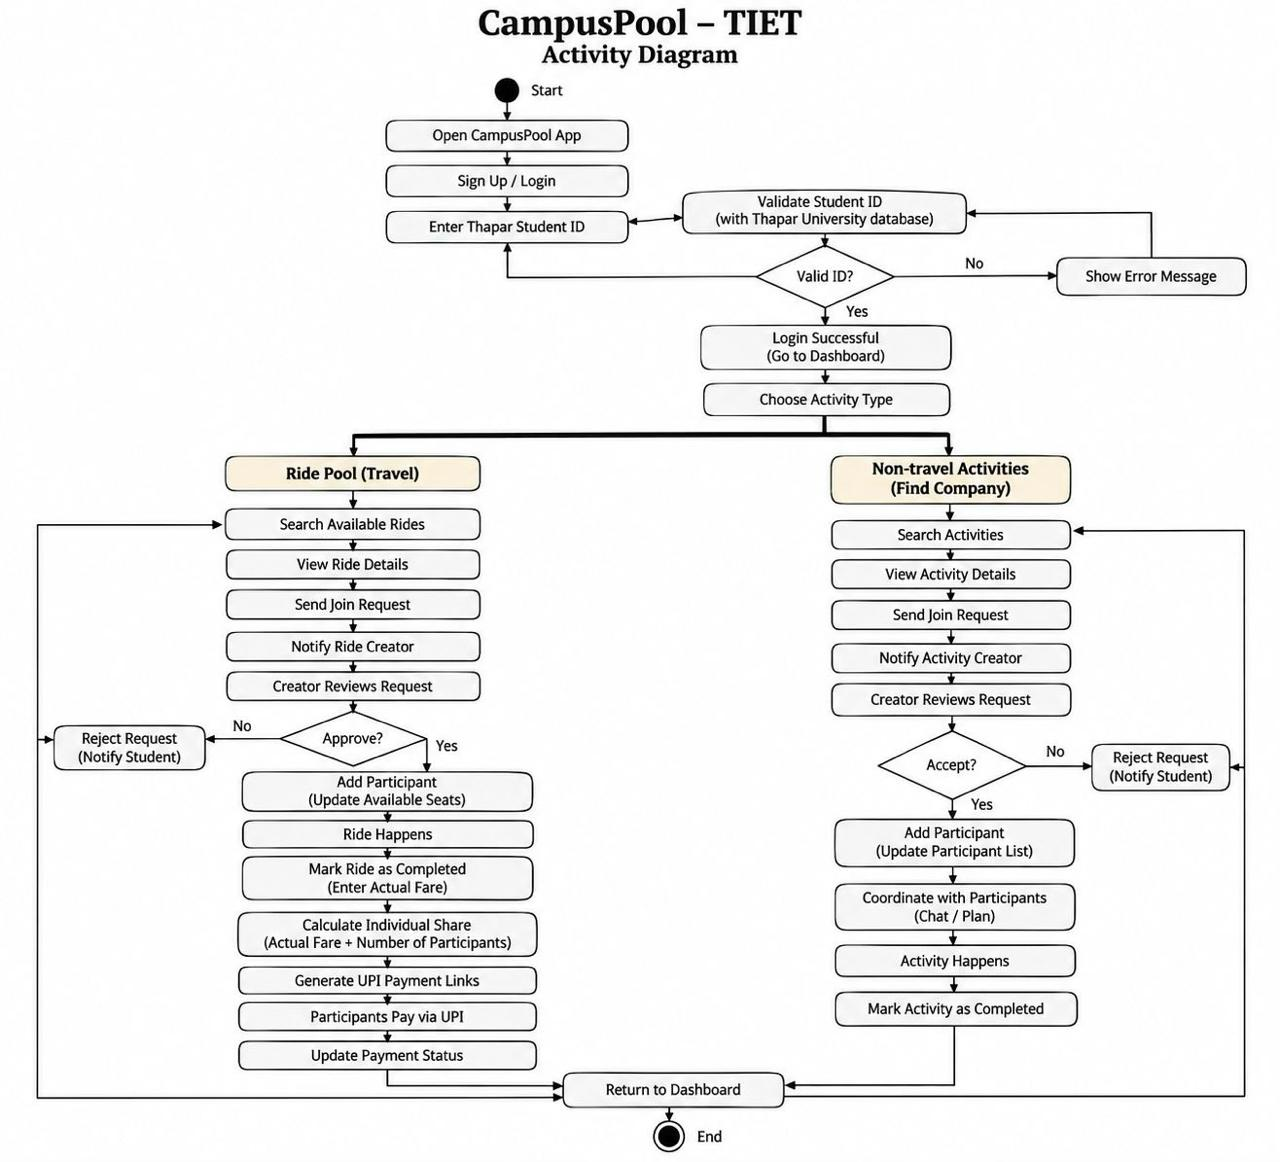
\includegraphics[width=\linewidth,height=.73\textheight,keepaspectratio]{activity-original.jpeg}\end{center}

\diagram{Swimlane diagram}{Responsibility is divided among the user, website, organiser and external services. Payment acknowledgement belongs to the rider, while receipt confirmation belongs to the organiser.}{swimlane-diagram.png}

\diagram{Conceptual class diagram}{The conceptual model groups users, plans, requests, membership, payments and reports. Student and Admin generalise to User. The implemented payment record stores a rider acknowledgement and a confirmed status.}{class-diagram.png}

\diagram{Data flow diagram Level 0}{The context diagram shows exchanges with users, organisers, administrators and the email service. UPI links launch an external application, while acknowledgement and confirmation return through website actions.}{dfd-level-0.png}

\diagram{Data flow diagram Level 1}{Account access, plan management, request decisions and fare tracking form the main logical processes. Stores D1--D6 describe logical data responsibilities.}{dfd-level-1.png}

\diagram{Data flow diagram Level 2}{The decomposed processes explain creation, search, request review and settlement. Account access uses email and OTP. Settlement separately records rider acknowledgement and organiser confirmation.}{dfd-level-2.png}

\diagram{Sequence diagrams}{The six interactions cover account access, ride creation, discovery, approval, settlement and activities. The payment sequence records acknowledgement before organiser confirmation.}{sequence-diagrams.png}

\clearpage
\section{Conclusion}
CampusPool gives campus plans a structured lifecycle from publication to participation and completion. The website combines discovery and organiser-controlled requests with communication and fare tracking. Its implementation separates the user interface, API and persistence layers and provides a container-based deployment path. The design models and verification cases explain how the main workflows should remain consistent across users.

\section{References}
\begin{enumerate}
\item CampusPool source repository. \url{https://github.com/pihuuaneja/ucs503p-202627campuspool}
\item UCS503 semester project guidelines. \url{https://tiet-ucs503.github.io/semester-project/}
\item Team-provided CampusPool design report and diagrams.
\item I. Sommerville, \emph{Software Engineering}, 10th edition, Pearson, 2015.
\item Object Management Group, \emph{Unified Modeling Language}, version 2.5.1, 2017.
\end{enumerate}
\end{document}
